% ==============================================================
% File     : chapters/04-MASArchitecture.tex
% Date     : 03 Apr. 2022
% Revision : 30 July 2022
% Creator  : Marco Peressutti
% ==============================================================


\chapter{MAS Architecture}
\minitoc

So far we have considered the main mechanisms of MASs: negotiation, communication and coordination.\\
But in these chapter we will focus on the technological aspect of MASs: how to build a system that employ such characteristics and mechanisms.

The context of MASs widens the notion of inteligent agents in two ways:
\begin{itemize}
\item An agent's user that imparts goals to it and delegates tasks might be not only human, but also another agent
\item An agent6 must be desifgned with explicit mechanisms of communicating and interacting with other agents
\end{itemize}
This new notion of intelligent agents needs to be taken into account when analysizing the general architecture of a MAS.

Formally:
\say{the infrastructure for a MAS is a set of services, conventions and knowledge that support complex social interactions (e.g. negotiations, agree on commitments...)}
Among the services that a MAS architecture can support we can find the following

\begin{figure}[!h]
\centering
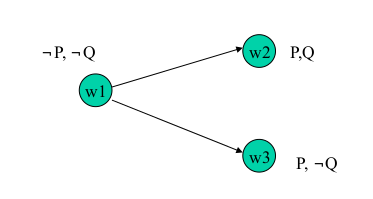
\includegraphics[width=.6\textwidth]{04/00}
\end{figure}

However, this is not a standard architecture, but rather a reference architecture that we can use in order to understand the kind of structures that can be included.\\
In particular, the structure of this architecture was proposed as a multi-layered architecture which includes a \side{MAS Infrastructure} and a \side{Individual agent infrastructure}.

\section{Low-level architectures}
The low level of the proposed architectures/set of services, deals with communication and the communication infrastructure. And there are only two ways that this infrastructure can be implemented: Shared memory and message sending/passing.
In the former, we consider how we can communicate via some common  channel where everybody can read and write something. In the latter, one agent send a message to exactly the recipient(s).

This is two basic approaches that can be implemented in very different ways and at different levels.
\subsection{Blackboards}
A possible shared memory approach to MAS communication there is a \side{Blackboard Architecture}.\\
The metaphor at the core of this architecture is that a collection of intelligent agents gather around a blackboard, loot at pieces of information written on it, think about them, and add their conclusions.

It means that each agent can only communicate via the blackboard.

Some basic assumptions of this method are 
\begin{itemize}
\item all of the agents can see all of the blackboard all the time, and what they see represents the current state of solution.\\
All information in the blackboard is available to all agents.
\item any agent can write his conclusions on the blackboard at anytime without gettin in anyone else's way.\\
The write operation is atomic and asynchronious.
\item the act of an agent writing on the blackboard will not confuse any other agents as they work.
\end{itemize}
The idea of blackboard architecture was originally implemented for translation of natural language.

The key ideas of the blackboard architecture is that problem solving should be:
\begin{itemize}
\item \side{Incremental}: complete solutions are constructed piece by piece, first hypothesizing a partial solution based on incomplete data and then attempting to verify additional data to verify hypothesis.\\

Agents do not just write whatever they want but rather they try to solve a problem (the solution to the problem is constructed incrementally).
\item \side{Opportunistic}: the system chooses the actions to take next that it determines will allow it to make the best progress towards meeting its goals in the current situation.\\

Having just a blackboard is not enough to solve a given problem, but there must be some organization mechanism on how to read, write and choose the next action. In other terms in order to solve the problem, the MAS must choose the most informative and useful element written in the balckboard
\end{itemize}
In figure \ref{fig:0401} a schematic representation of the blackboard architecture is proposed.
\begin{figure}[!h]
\centering
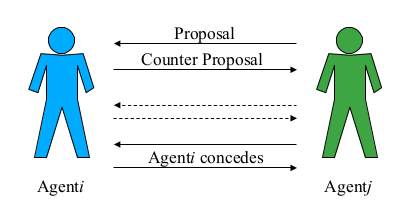
\includegraphics[width=.5\textwidth]{04/01}
\caption{}
\label{fig:0401}
\end{figure}

From the basic representation of the blackboard architecture we can identify the following main components:
\begin{itemize}
\item A \side{blackboard}: a global database containing data and hypotheses (potential partial solutions). 
\item A set of \side{Knowledge Sources (KS)} or agents
\item A \side{Control mechanism}, which will say what happens after an agents write something on the blackboard or that will decide who is going to be the next source of information.
\end{itemize}

The main control problem then is that of selecting the best action to execute next.

Blackboard systems, in fact, must have some control mechanism:
\begin{itemize}
\item allow effective control requires to take into account
\begin{itemize}
\item \side{Goal-directed factors}: based on what an agent wants.
\item \side{Data-oriented factors}: based on what an agent is best able to do. (based on what is written in the blackboard)
\end{itemize}
\item Blackboard control is difficult because it can be difficult to determine the expected value of an action by an agent as there may be complex interrelationships among the agents.
\end{itemize}

Before going into depth of the application of the blackboard architecture there is one important hypothesis that need to be considered: the \side{Serialisation Hypothesis}.\\
In principle, the idea is that agents can read and write whenever they want, but this is not efficient because there must be some kind of order in which agents can do this. \\
Such order is ensured by some serialisation:
\begin{itemize}
\item agents are schedulable entities and only one can be running at any time.
\item The control mechanism selects only the most productive agent at any given moment to work on the problem.
\item The blackboard is not gloabally visible. Agents generally work on a limited area of the blackboard, known as the agent's context.

In fact in principle agents have access to all the information of the blackboard, however for an efficiency point of view, it is better if agents look only into some locations.
\item Implicit assumption: a knowledge source/agent operates within a valid, or consistent context.
\end{itemize}

\subsubsection{Agenda-based Control}
A first type of Blackboard architecture that we consider is the \side{Agenda Base Control}.
\begin{figure}[!h]
\centering
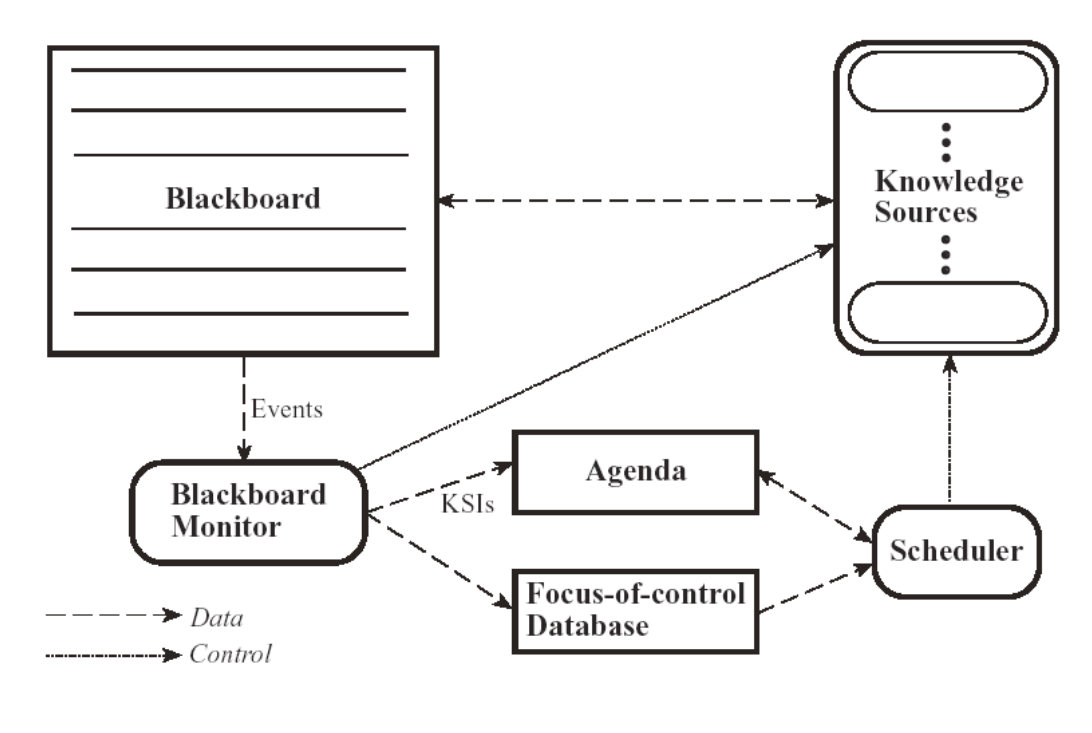
\includegraphics[width=.5\textwidth]{04/02}
\end{figure}
\begin{enumerate}
\item Each agent can write into Blackboard, and the act of writing generates some event. 
\item The event is then processed by some Blackboard monitor: a component that monitor what is going on in the blackboard and what should be the reaction.
\item When something new happears, the Blackboard monitor select what are other agents to whom this information may be useful.\\
\item Such information will be sent directly to the selected agents as a part of a preconditions for their execution. 
\item The selected agents will be put into an agenda to be scheduled for execution.
\item They way agents are selected from the agenda is through a rating which is attributed to each agent via a Focus-of-control database .\\
The task of this component  is to rate the execution of agents in the agenda based on the information and some other criteria.
\end{enumerate}
In the basic agenda-based blackboard architecture, all the control (strategy) knowledge of the system is represented in a single scheduler rating function.\\
This makes it difficult to encode and modify complex control strategies.\\
The knowledge and reasoning are not explicit.

\subsubsection{Event-based Control}
There are some alternative and modification of this type of control. When there may be not just one but many Event list that are triggered by the blackboard.
\begin{figure}[!h]
\centering
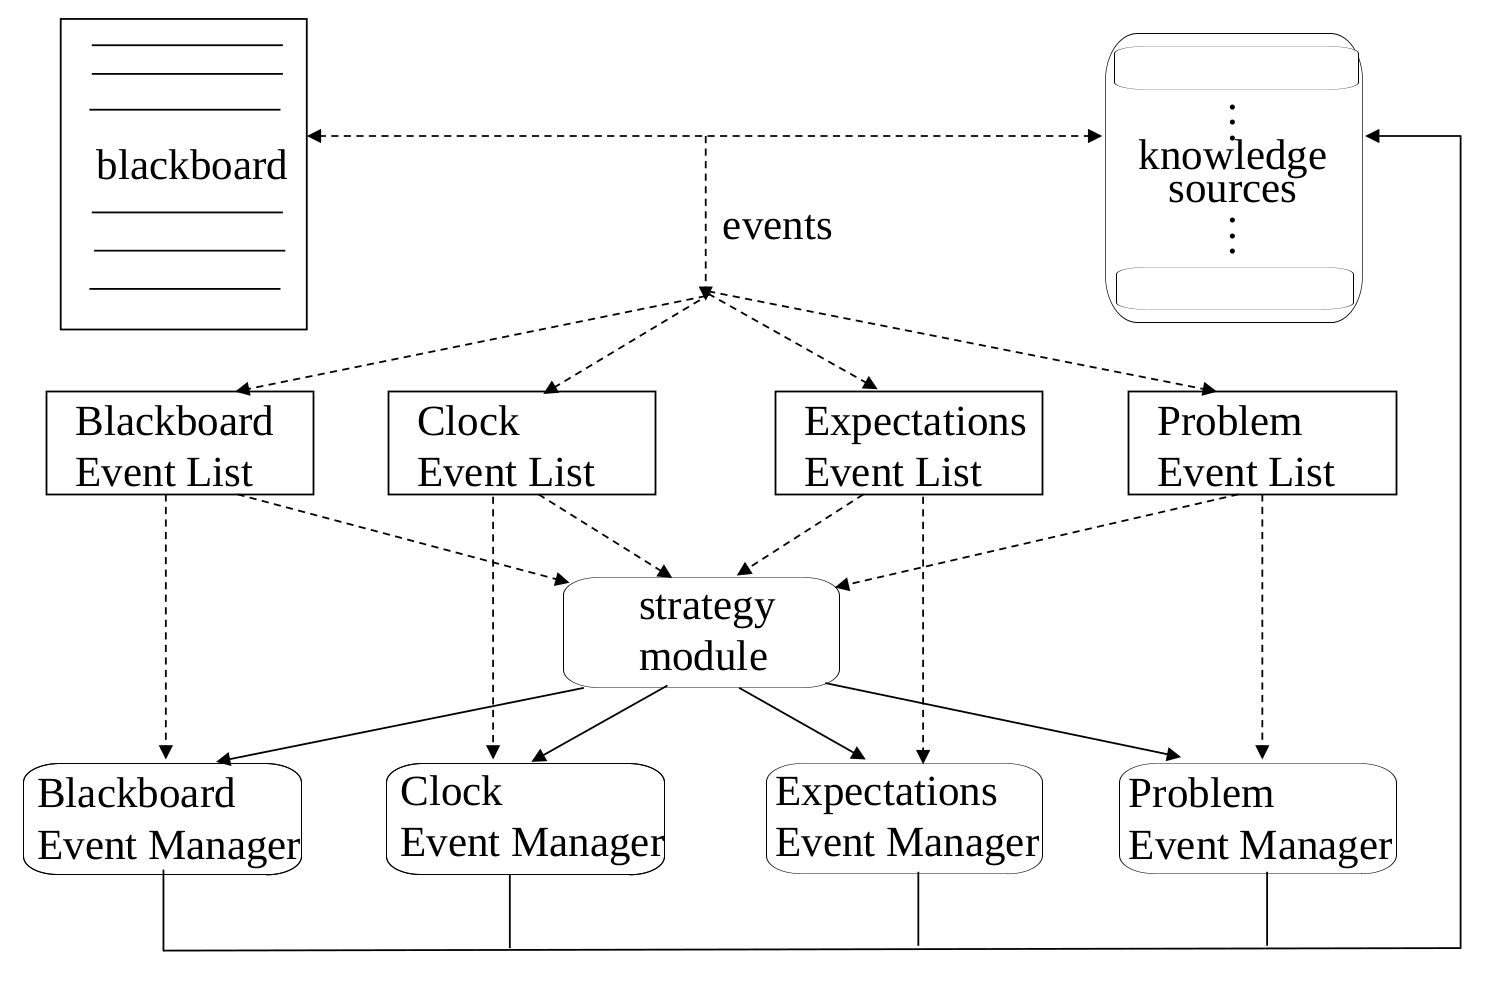
\includegraphics[width=.5\textwidth]{04/03}
\end{figure}
\begin{enumerate}
\item An agent write to the blackboard and an event is generated
\item Such event is then classified based on some property. This differentiate and classify what the agents is writing on the blackboard, which might be a general information, an expectation or a problem.
\item From the chosen amount of blackboard monitor there will be some strategy module, who decides from which event list to choose from.
\item A particular monitor/manager will handle the resulting event and transmit it to knowledge sources.
\end{enumerate}

\subsubsection{Goal-directed Control}
\side{Goal-directed control} considers the role and the ultimate value of actions in satisfying the system's goals.

\begin{figure}[!h]
\centering
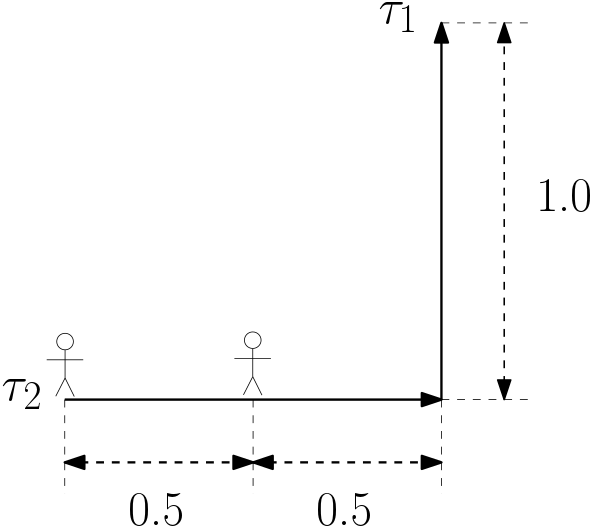
\includegraphics[width=.5\textwidth]{04/04}
\end{figure}
In this case there are two blackboard, namely a \side{Domain Blackboard} and a \side{Goal Blackboard}

\begin{enumerate}
\item An agent writes on the Domain Blackboard and generates an event
\item The goal processor processes information in the blackboard and transmit it to a particular agent and schedule such agent to execute via a scheduler.\\
In addition, the goal processor maps the event into a goal balckboard, whenever it cannot identify a specific agent to convey such information to.\\
From the goal blackboard some subgoals can be generated until an agent is found according to what we need.

This is some sort of reasoning mechanism that yields a more elaborated processing of each goal.
\end{enumerate}

Goal processor instantiates goals on the goal blackboard. Goal processor is driven by the 3 mapping functions. Integrates goal-directed and data-directed factors:
\begin{itemize}
\item Goal-directed goals are created in response to the creation of other goals based on the goal-to-subgoal map
\item Data-directed goals are created in response to the creation or modification of hypotheses on the blackboard based on the hypothesis-to-goal map
\end{itemize}

When a goal is inserted onto the goal blackboard, it may trigger KSs that can achieve the goal identified by the goal-to-KS map.\\
If KS is likely to generate a hypothesis to achieve the goal, KS is added to the agenda.\\
A possible problem may emerge: subgoaling needs to be carefully controlled.



\subsubsection{Hierarchy of Blackboard Servers}
Moreover, we can consider that the blackboard architecture is in reality a distributed blackboard, since keeping a centralized blackboard for every agent in the MAS can be a bottleneck.

However, by creating an hierarchy or a distributed system of blackboard. Between which some relations and dependecies exist.

\begin{figure}[!h]
\centering
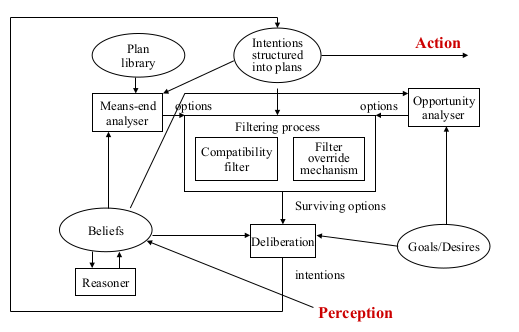
\includegraphics[width=.5\textwidth]{04/05}
\end{figure}

Whenver a goal gets written into a blackboard but there are no sources that can be find to understand what the next action should be, it will be forwarded to the upper level blackboard.
Such parent blackboard will see information and identify a blackboard that can process the information.
If yet there is no one that can process the information it will forward the goal to its parent blackboard and repeat the process.

\subsection{ACTORs}
ACTOR model approach is a pure message passing architecture that has the following properties
\begin{itemize}
\item \side{Social}, can send messages to other ACTORs
\item \side{Reactive}, carry out computation in response to a message received from another actor
\end{itemize}
In the ACTOR model, computation itself is viewed as message passing.
It can be considered as consisting of:
\begin{itemize}
\item An address
\item A behaviour which specifies what the ACTOR will do upon receipt of a message
\end{itemize}
In other term, we have some agents to be considered as a reactive entity, that has an address and a behaviour. Whenever an agent receives a message it executes its behaviour. As such agents are programs that can be triggered and have some address that we can invoke directly.

The ACTOR approach is formulated around three main design objectives:
\begin{enumerate}
\item Shared, mutable data. \\
Not shared channel but shared channels. This can be some kind of common data that all agents need in order to perform some kind of communication.
\item Reconfigurability.\\
New agent can be created and it is possible to communicate with such new agents.
\item Inherent concurrency.\\
Asynchronius behaviour is possible.
\end{enumerate}

An ACTOR is an object that carries out its actions in response to communication it receives.\\
ACTOR may perform only three basic actions:
\begin{itemize}
\item Sending messages to itself or other ACTORs
\item Creating more ACTORs
\item Specify a replacement behaviour, which is essentially another actor that takes the place of the actor that creates it, for the purpose of responding to certain communications.
\end{itemize}

The behaviour of an ACTOR model system is as follow:
\begin{itemize}
\item Upon receipt of a message, the message is matched against the ACTOR's behaviour (script)
\item Upon a match, the corresponsing action is executed, which may involve:
\begin{itemize}
\item Sending more messages
\item Creating more ACTORs
\item Replacing the ACTOR by another
\end{itemize}
\end{itemize}

ACTOR computation is therefore reactive.\\
An ACTOR is dormant until it receives communication.\\
In any computation, each ACTOR receives a linearly ordered sequence of computations.\\
Messages are not guaranteed to arrive in the order in which they are sent\\
There is no assignment to local variables in basic actor model\\
Every communication must be sent to a mail address: mail system is an important part of the model.

The communication event in actor model is called a task and it has 3 parts:
\begin{enumerate}
\item A unique tag, distringuishing it from tasks in the system
\item A target, the mail address of intended receiver
\item A communication which is the data passed by this communication event
\end{enumerate}

Actor model is asynchronous.\\
Communication is:
\begin{itemize}
\item explicity, through mail addresses, without shared variables 
\item buffered and asynchronous
\end{itemize}
Weak fairness is assumed:
\begin{itemize}
\item every message which is sent is eventually delivered
\item every computation eventually progress (no starvation)
\end{itemize}

\begin{figure}[!h]
\centering
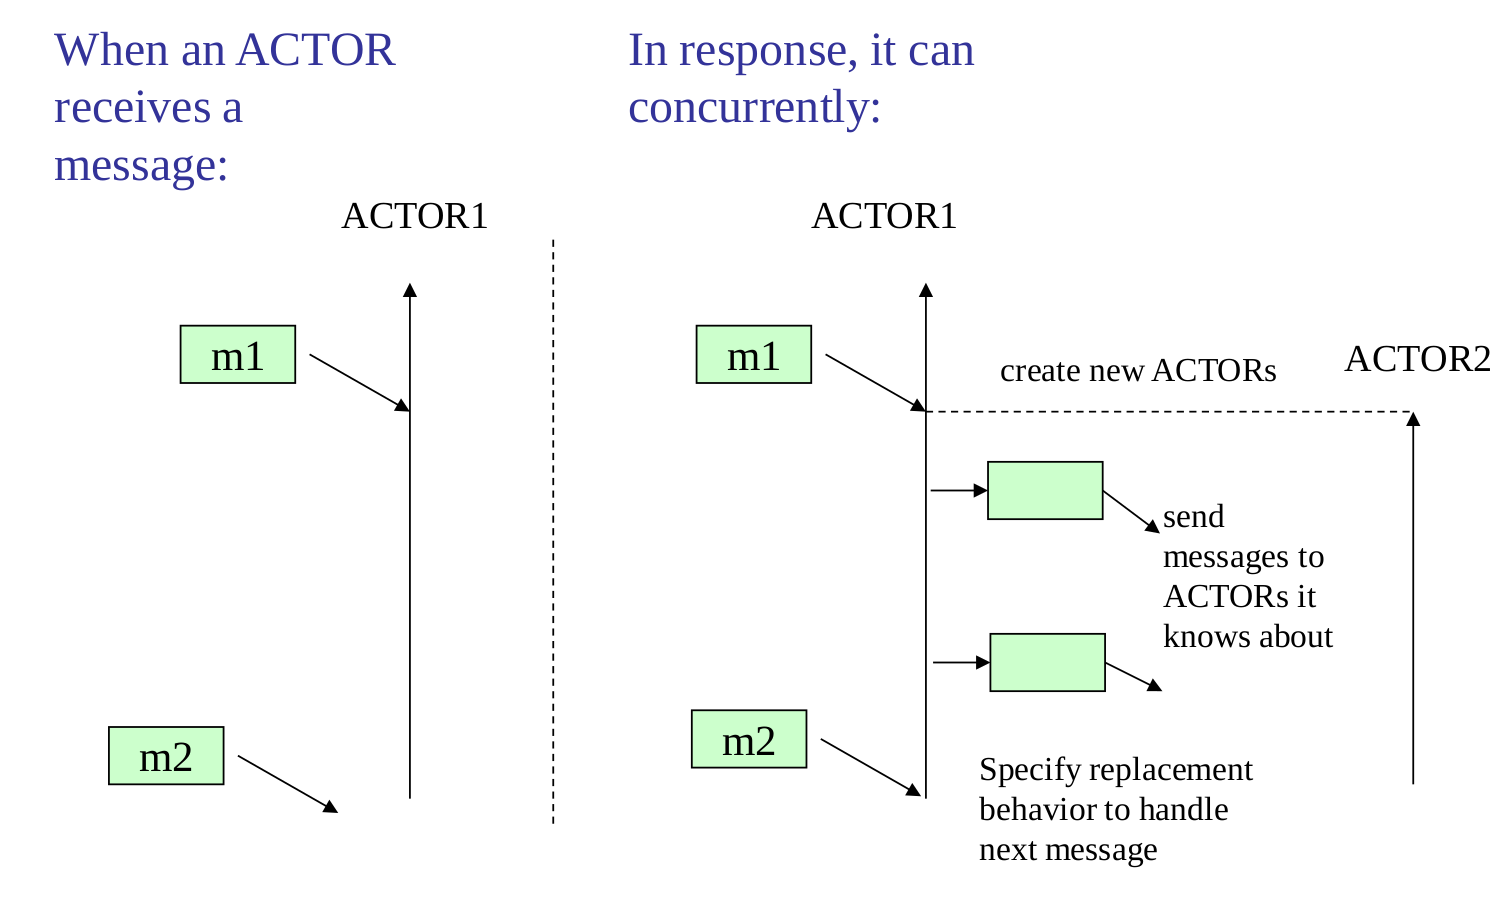
\includegraphics[width=.5\textwidth]{04/06}
\end{figure}


\subsubsection{Message sending based architecture: Agent Factory}
A few words about basic principles of Agent Factory:
\begin{itemize}
\item Linear discrete model of time which can be visualized as a sequence of numbers
\item A guaranteed delivery assumption. Messages are delivered correctly: the content of the message does not change in transaction, the message is sent to destinations and only to them
\item For any message there is only one sender
\item In spite of process synchronization: communication is asynchronous via message pool
\end{itemize}

\begin{figure}[!h]
\centering
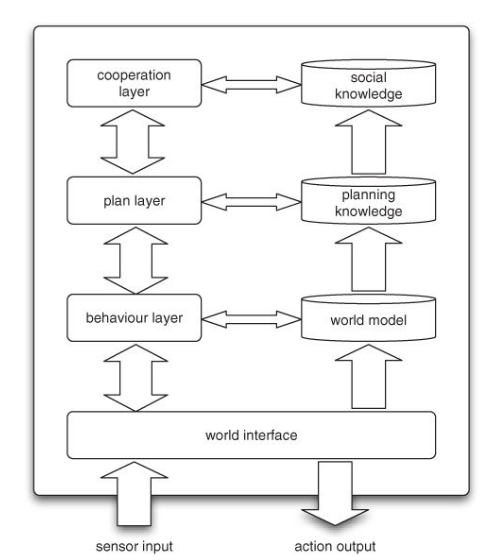
\includegraphics[width=.5\textwidth]{04/07}
\end{figure}

\section{Testbeds}
\side{Testbeds} are high-level architectures, which where developed specifically in the DAI community.\\
The main purpose of DAI testbeds is to support the implementation of ideas so that they can be evaluated in a useful context. In other terms, if a designer would like to propose a new algorithm for communication and negotiation, it can compare it with other algorithms via a testbed: this will allow to use the same example, the same tasks and the same system.

In order to have such a possibilities most DAI testbeds provide three classes of facilities to compare different class of algorithm:
\begin{itemize}
\item \side{Domain facilities}: representation and simulation of the problem being solved
\item \side{Development facilities}: an environment or tools for building the agents that will solve the problem
\item \side{Evaluation facilities}: tools for display, data collection, and analysis to understand how well the agents perform
\end{itemize}

\subsection{DVMT}
The \side{Distributed Vehicle Monitoring Testbed (DVMT)} is a DAI testbed developed to successfully track a number of vehicles that pass within the range of a set of distributed sensors (agents).

\begin{figure}[!h]
\centering
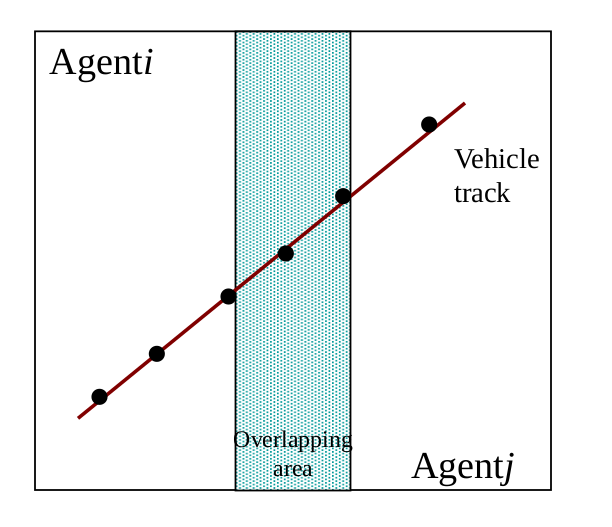
\includegraphics[width=.5\textwidth]{04/11}
\end{figure}

DVMT is a problem dependent testbed and agents (problem solvers) have a blackboard architecture.

\subsection{MACE}

MACE provides tools for constructing DAI systems at different level of abstraction with agents that have an ACTOR model:
\begin{itemize}
\item Each rule can be an agent
\item coarse-grained systems with large scale agents
\end{itemize}
MACE had no fixed domain for problem solving activity, however it have some fixed examples. 

\section{Infrastructures that use wrappers: ARCHON}
In many industrial applications, a substantial amount of time, effort and money was spent on developing complex and shophisticated software systems (e.g. expert systems and databases).\\
The basic idea is that we have a legacy system and we would like that these systems operate in a new environment. In order to do so, the designer could provide them with a wrapper that enable them to use in any other agent system.

This is what was implemented in \side{ARchitecture for Cooperative Heterogeneous ON-line systems (ARCHON)} was (in 1996) Europe's largest project in the area of DAI.\\
It was originally focused on getting a number of expert systems to pool their expertise in solving problems and diagnosing faults in several industrial domains.\\
Supports a cooperating community that has decentralized control and individual problem solving agents.\\
Consists of a:
\begin{itemize}
\item \side{Framework}: which provides assistance for interaction between constituent subcomponents
\item \side{Methodology}: which provides a means for structuring these interactions
\end{itemize}

ARCHON's individual problem solving entities are agents; they have the ability to control their own problem solving and to interact with other community members\\
Agents are large grain loosely coupled and semi-autonomous.\\
Each agent consists of an \side{ARCHON Layer (AL)} and an application program (known as \side{Intelligent System (IS)})\\
The ISs can be heterogeneous as their differences are masked by a standard AL-IS interface.\\

\begin{figure}[!h]
\centering
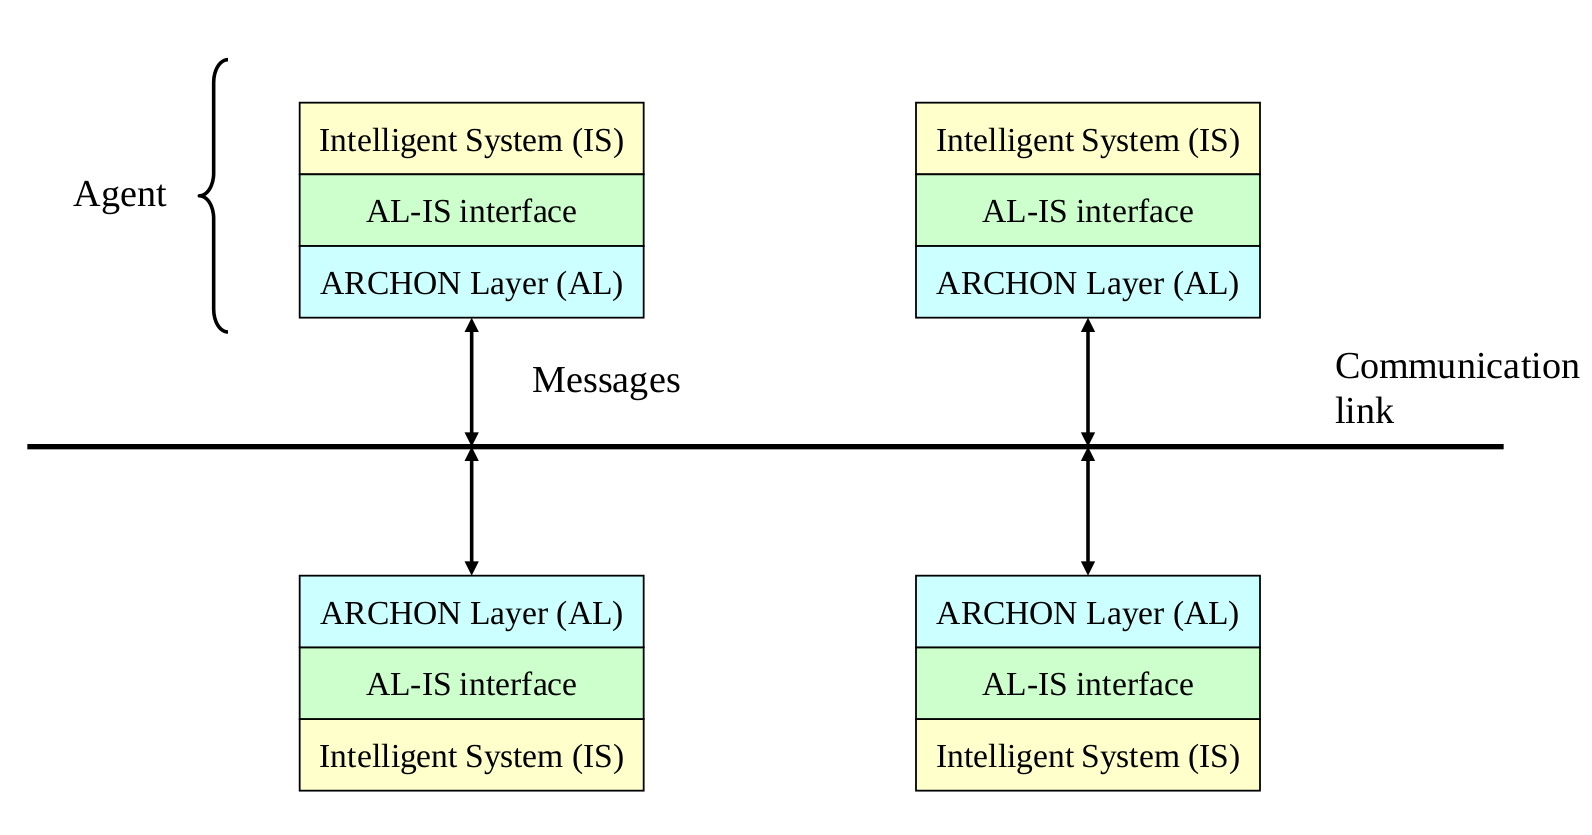
\includegraphics[width=.5\textwidth]{04/08}
\caption{}
\label{fig:archoncommunity}
\end{figure}

Figure \ref{fig:archoncommunity} shows the basic ARCHON community structure. Each agent has an:
\begin{itemize}
\item ARCHON layer that is responsible for the implementation of interagent communication and other services that are necessary for communication
\item An interface layer that allow the designer to wrap the Intelligent System into the overall MAS.
\end{itemize}
Communication happens via a single communication link or bus. This is fairly similar to KQML system where the Archon layer was the router, the AL-IS interface is similar to KRIL and lastly the intelligent system was the system itself.

This is a more general way of implementing a communication system where we define a set of general features that can be used by other system to communicate with the ARCHON Layer. This implies that it does not matter how we implement our Intelligent System, the communication will be consistent.

The most interesting part is how the AL-IS interface is structured, because it does not consist of a simple API, but more advanced techniques.

The system's overall objective is expressed in the separate local goals of each agent.\\
Agents' goals are usually interrelated. Therefore, social interactions are required to meet gloabl contraints.\\
Such interactions are controlled by the ARCHON layer which functions are to:
\begin{itemize}
\item Control tasks within the local IS
\item Decide when to interact with other agents (it needs to model the capabilities of its own IS as well the ISs of the other agents)
\item Communicate with other agents
\end{itemize}

\begin{figure}[!h]
\centering
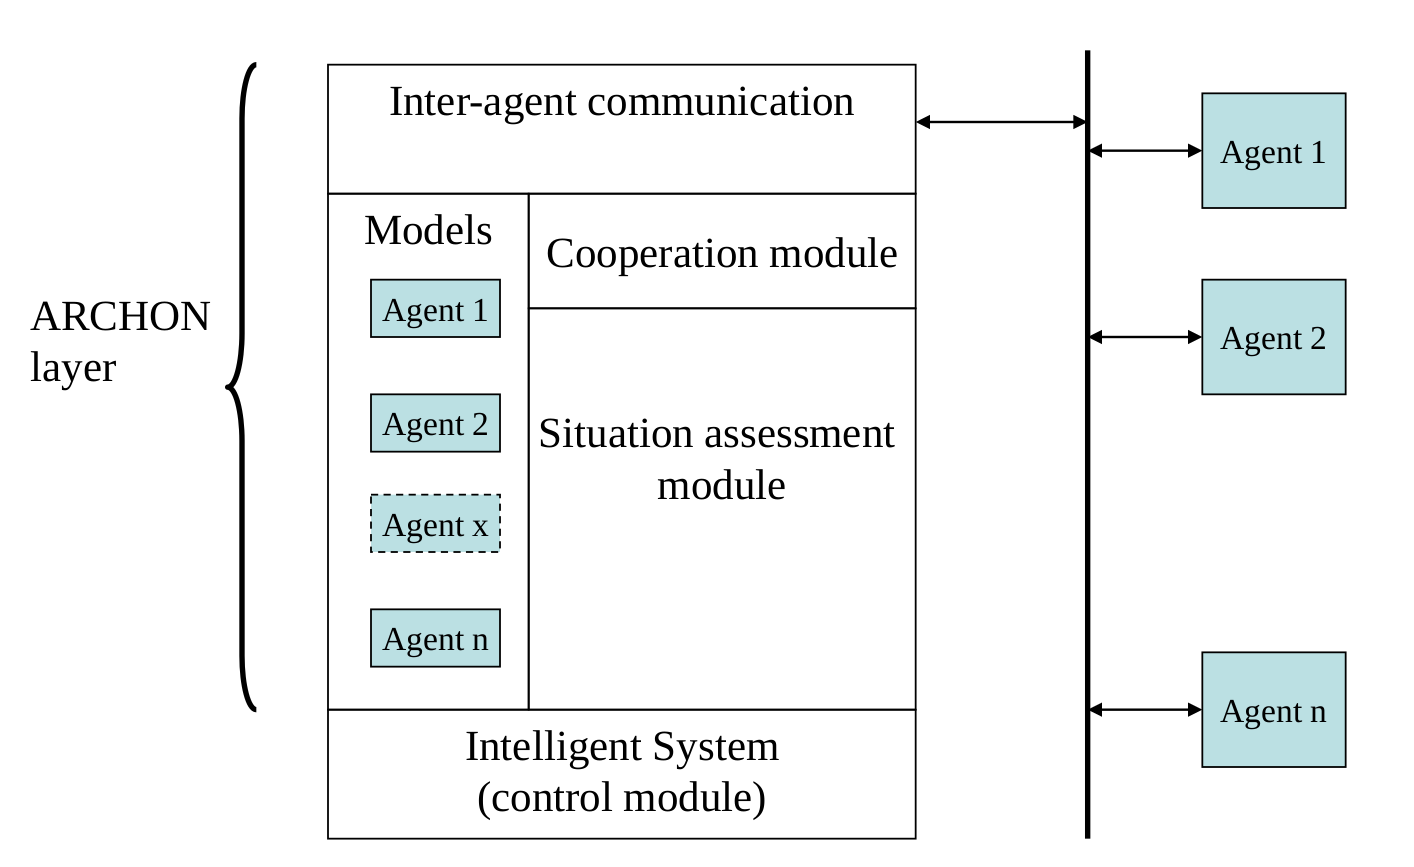
\includegraphics[width=.5\textwidth]{04/09}
\end{figure}

Looking into the three basic layers of the ARCHON architecture/approach we can notice that the ARCHON Layer can be devided into several modules:
\begin{itemize}
\item An Inter-agent communication layer/module that is responsible for supporting communication
\item An interface which is a set of components that can be adjusted in order to plugin the Intelligen System.

Among these modules we might find a \side{Cooperation module}, a \side{Situation assessment module} (something that you can tune in order to adjust your system), a set of Models of other agents or of itself.
\end{itemize}

In other terms this is a basic implementation that you can adjust in order to plugin the desired legacy system or intelligent system. It is a smooth translation model to some generic agent architecture.

\section{Infrastructures that use Middle Agents: RETSINA}
The idea of Middle agents is that instead of having a direct mechanism, Middle agents is a highly intelligent blackboard that it is implemented as shared memory but rather as an agent that can keep relationships between tasks and requests and proposals.

\begin{figure}[!h]
\centering
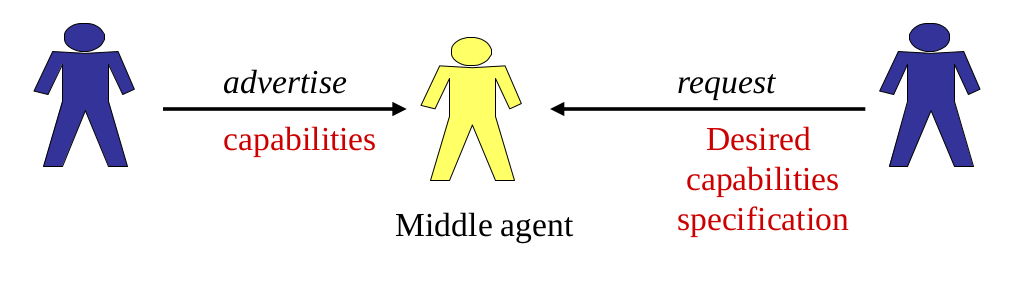
\includegraphics[width=.5\textwidth]{04/10}
\end{figure}

In an open system, the set of agents is not known a priori.\\
The infrastructure should provide ways for its agents to locate each other based on name, functionality or capability.

Agents that provide this service are called Middle agents which may also take the role of Facilitators or Matchmakers.

\side{REusable Task Structure-based Intelligen Network Agents (RETSINA)} is an open MAS infrastructure that supports communities of heterogeneous agents.\\
The main idea of RETSINA is that agents should form a community of peers that engage in peer-to-peer relations.\\
There is no central control and it implements distributed infrastructural services that facilitate the relation between agents.

RETSINA actually implements all the layers proposed in the reference architecture at the beginning of this chapter except for the interoperation layer.

\begin{figure}[!h]
\centering
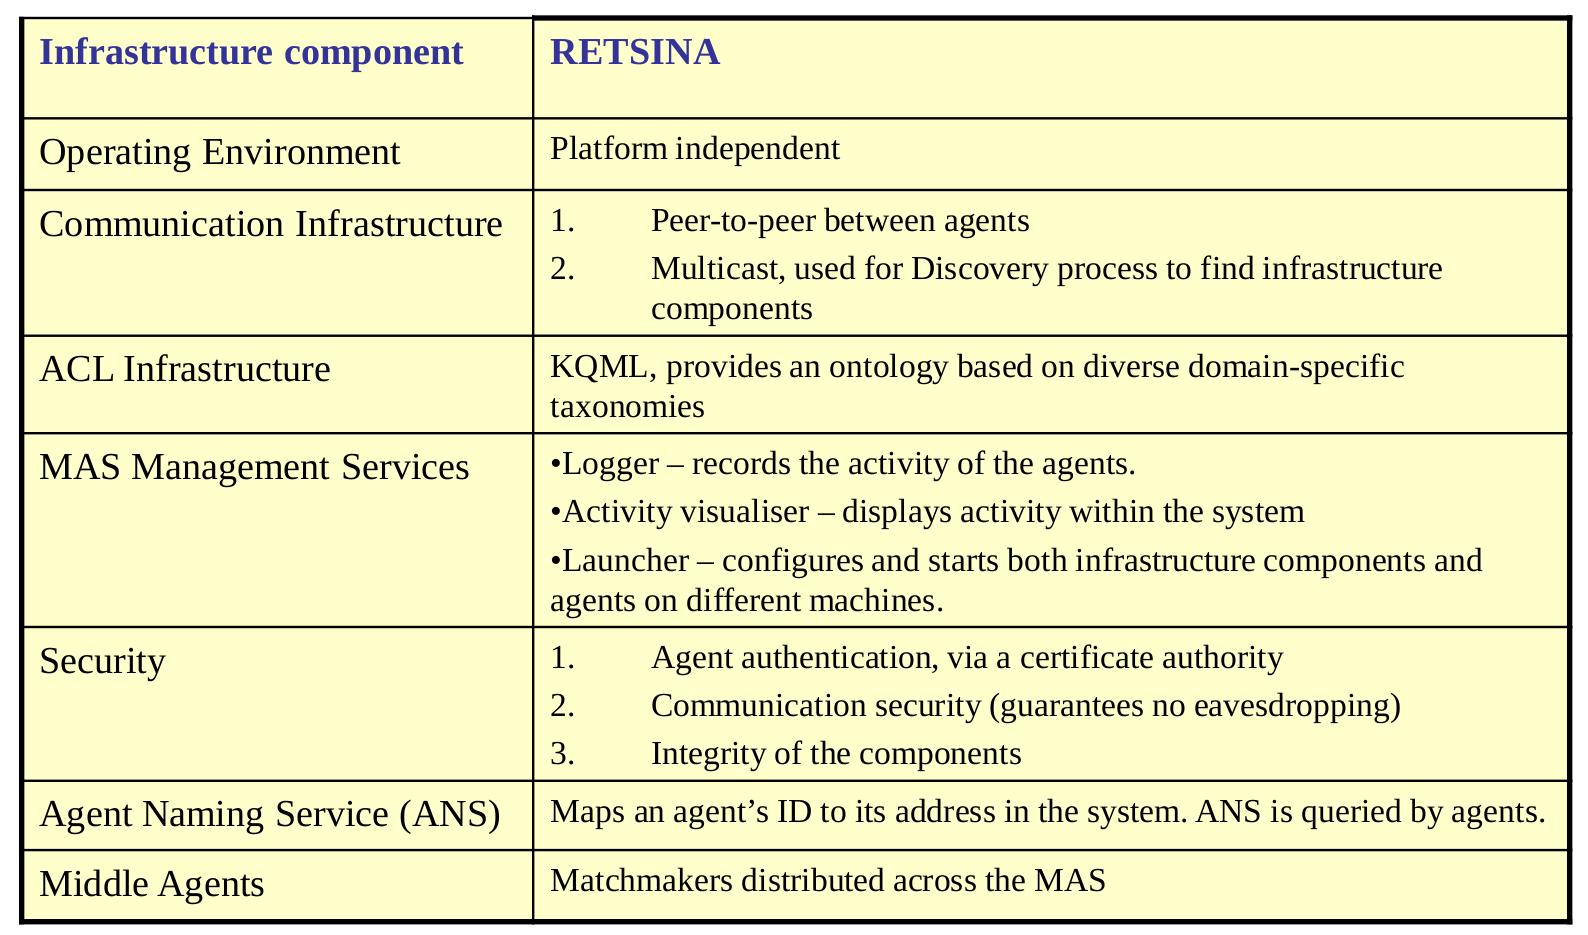
\includegraphics[width=.8\textwidth]{04/12}
\end{figure}

RETSINA middle agents are called Matchmakers, i.e. information agents that look for other agents rather than information:
\begin{itemize}
\item Records a mapping between agents in the system and the services they provide
\item Two types of data: advertisements and requests
\item the task of matchmakers is to match advertisements to requests
\item Two types of protocols: single shot and monitor
\end{itemize}


\section{Market-based architectures}
Online market places offer an opportunity to buyers and sellers to meet electronically and conduct trade. In some sense, these architecture consider a Middle agent to conduct their activity, but a special one which is the market place itself.

Offers benefits for both buyers and seller:
\begin{itemize}
\item Buyers: ease to process of searching for and comparing sellers
\item Sellers provide access to much broader customer bases
\end{itemize}

The major challenges are:
\begin{itemize}
\item to go beyond simple buying and selling
\item to incorporate time constraints, enforce deadlines, interact with a highly distributed web of suppliers with different capabilities and resources, interact over long periods of time and deal with failure in contract execution
\end{itemize}

The requirements of a Market-based Architecture are to:
\begin{itemize}
\item Provide support for a variety of transaction types (buying and selling, complex multi-agent contract negotiation, auctions)\\
This mechanism should be oriented towards different type of transactions.
\item Control fraud and misrepresentation
\item Discourage counterspeculation
\item Provide for secure and private credit and payment mechanisms
\item Provide a language in which the rich array of semanting content about commerce can be expressed
\item Provide for robust exception handling
\item Scale smoothly from local to global
\item Be extensible, by third parties
\item Interoperate with other new and existing electronic commerce services
\end{itemize}
So the idea is that in addition to the standard Matchmaking propose-request we need to implement the aforementioned features.

\subsection{MAGNET}
The  \side{Multi-AGent NEgotiation Testbed (MAGNET)} is a testbed to support multiple agents in negotiating contracts.\\
Supports negotiation of contract for tasks that have temporal and precedence constraints.\\
Distinguishes between the agents:
\begin{itemize}
\item Customer: needs resources outside its direct control in order to carry out its plans
\item Supplier: provides the resources and services required by customers, for a specified price, over specified time periods
\end{itemize}

\begin{figure}[!h]
\centering
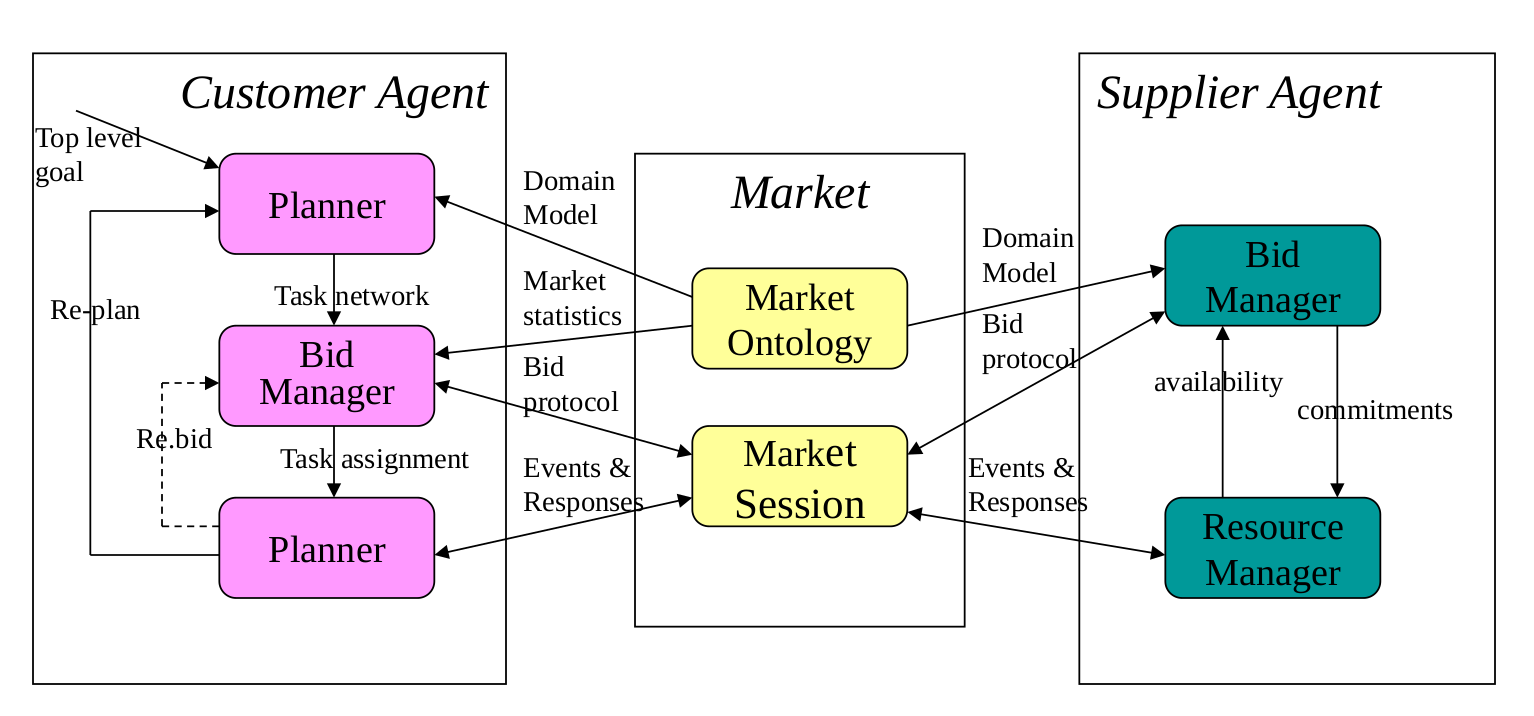
\includegraphics[width=.5\textwidth]{04/13}
\end{figure}

In this architecture there are:
\begin{itemize}
\item A special element called market that implements market sessions and may implement also Market Ontology or knowledge about such market place.
\item Customer agents, that are provided with a Planner in order to plan its task and a Bid Manager.
\item Supplier agent will have a Bid Manager and a Resource Manager.
\end{itemize}

In the general case, the bidding process goes as follows:
\begin{enumerate}
\item Customer agent plans a set of task
\item Getting information about the Market Ontology, the Customer Agent can create bids via the Bid Manager and publish such tasks to be performed into the Market Session
\item The Supplier Agent gets information about the Market Ontology and via the communication between the Bid Manager and the Resource Manager, decides which of the resources of interest are available.
\item Based on the information of availability derived from the Resource Manager, the Supplier Agent will publish into the Market Session
\item The bid protocol will coordinate the rules of the action or negotiation.
\item Depending on whether or not the bid was accepted or rejected, the Customer Agent may decide to rebid or replan its tasks.
\item Upon agreement the Supplier Agent will commit via the Resource Manager to provide the agent with the resources needed.
\end{enumerate}


The interaction among agents goes as follows
\begin{enumerate}
\item A customer issues a Request for Quotes (RFQ), which sp[ecifies tasks, the precedence relations and a timelien for the bidding process
\item Supplier agents submit a bid, which includes a set of tasks, a price, a portion of the price to be paid as a non-refundable deposit and estimated timeline
\item The customer decides which bid to accept based on cost, risk and time constraints
\item The customer awards bid, notifies the suppliers of their commitments and specifies the work schedule
\end{enumerate}

The interactions between the customer and supplier agents are encapsulated in a market session. The market session:
\begin{itemize}
\item finds suppliers interested in bidding for the customer
\item provides a catalog of services (market ontology)
\item time-stamps all the interactions in order to avoid dispute among customers and suppliers
\end{itemize}

\begin{figure}[!h]
\centering
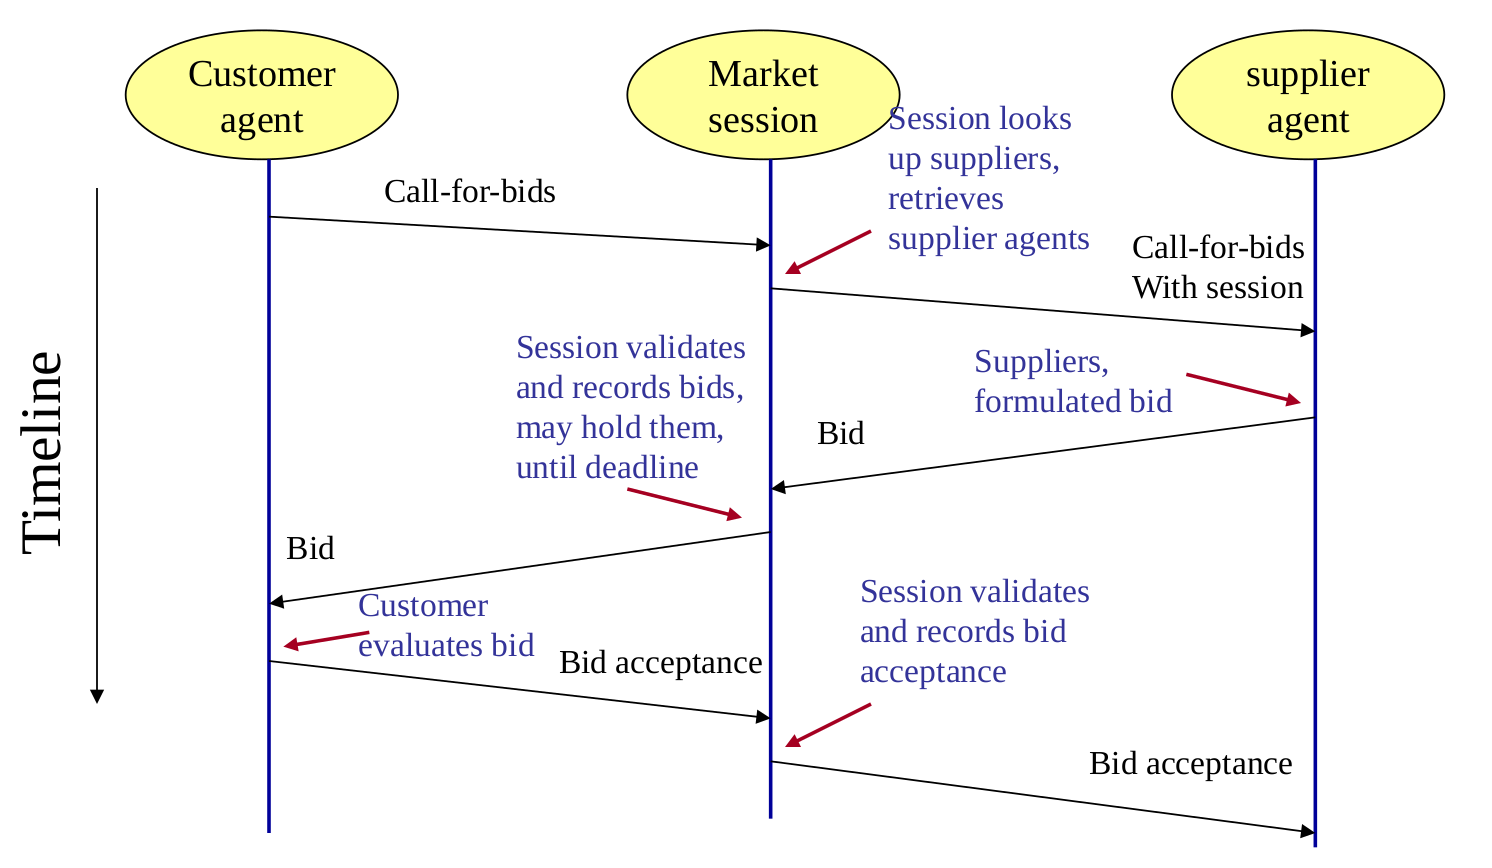
\includegraphics[width=.5\textwidth]{04/14}
\end{figure}

The session:
\begin{itemize}
\item Truthfully informs the suppliers of the conditions under which the bidding is being done and enforces these conditions
\item Can limit the number of bids sent by each supplier
\item May provide information about suppliers to customers
\item Enforces the rules of the market
\item Can act as a trusted auctioneer
\end{itemize}

\section{Conclusion}
We consider our MAS infrastructure as middleware on the top of system software.
Cooperative work support is an important element of the infrastructure and it needs conceptual solutions
Extensibility and default components are important features
We should be as much as possible close to standards (if they do not exist then to general tendencies)



